\documentclass{ctexart}
\usepackage{graphicx}
\usepackage{caption}
\usepackage{float}
\usepackage{amsmath}
\usepackage{fancyhdr}
\usepackage{xunicode-addon}
\usepackage{booktabs}
\usepackage[a4paper,hmargin=1.25in,vmargin=1in]{geometry}
% !TeX program = xelatex
\title{\begin{figure}[H]
	\centering 
	\includegraphics[height=7cm,width=14cm]{E:/Pictures/中科大.jpg}
	\end{figure}\Huge\textbf{Lab 2}\\\huge{Python爬虫实验}}
\date{}
\punctstyle{banjiao} 
\pagestyle{fancy}
	\fancyhead[C]{\LARGE\textbf{Report 2}}
	\fancyhead[L]{}
	\fancyhead[R]{}
	\fancyfoot[C]{\thepage}
\begin{document}
	\maketitle
	\thispagestyle{empty}
	
	\[\makebox{\Large{姓名:\underline{\makebox[5cm]{高茂航}}}}\]
	
    \[\makebox{\Large{学号:\underline{\makebox[5cm]{PB22061161}}}}\]
	
	$$\makebox{\Large{日期:\underline{\makebox[5cm]{2024.3.21}}}}$$
	
	\clearpage

	\pagenumbering{arabic}
    \section{Task1}
    \subsection{Algorithm Description}
	使用\verb|urllib.request.urlopen().read()|提取网页的html文件,然后用\verb|decode()|函数将html文件转为文本文件并写入\verb|page.txt|文件。

\subsection{Results}
\begin{figure}[H]
	\centering 
	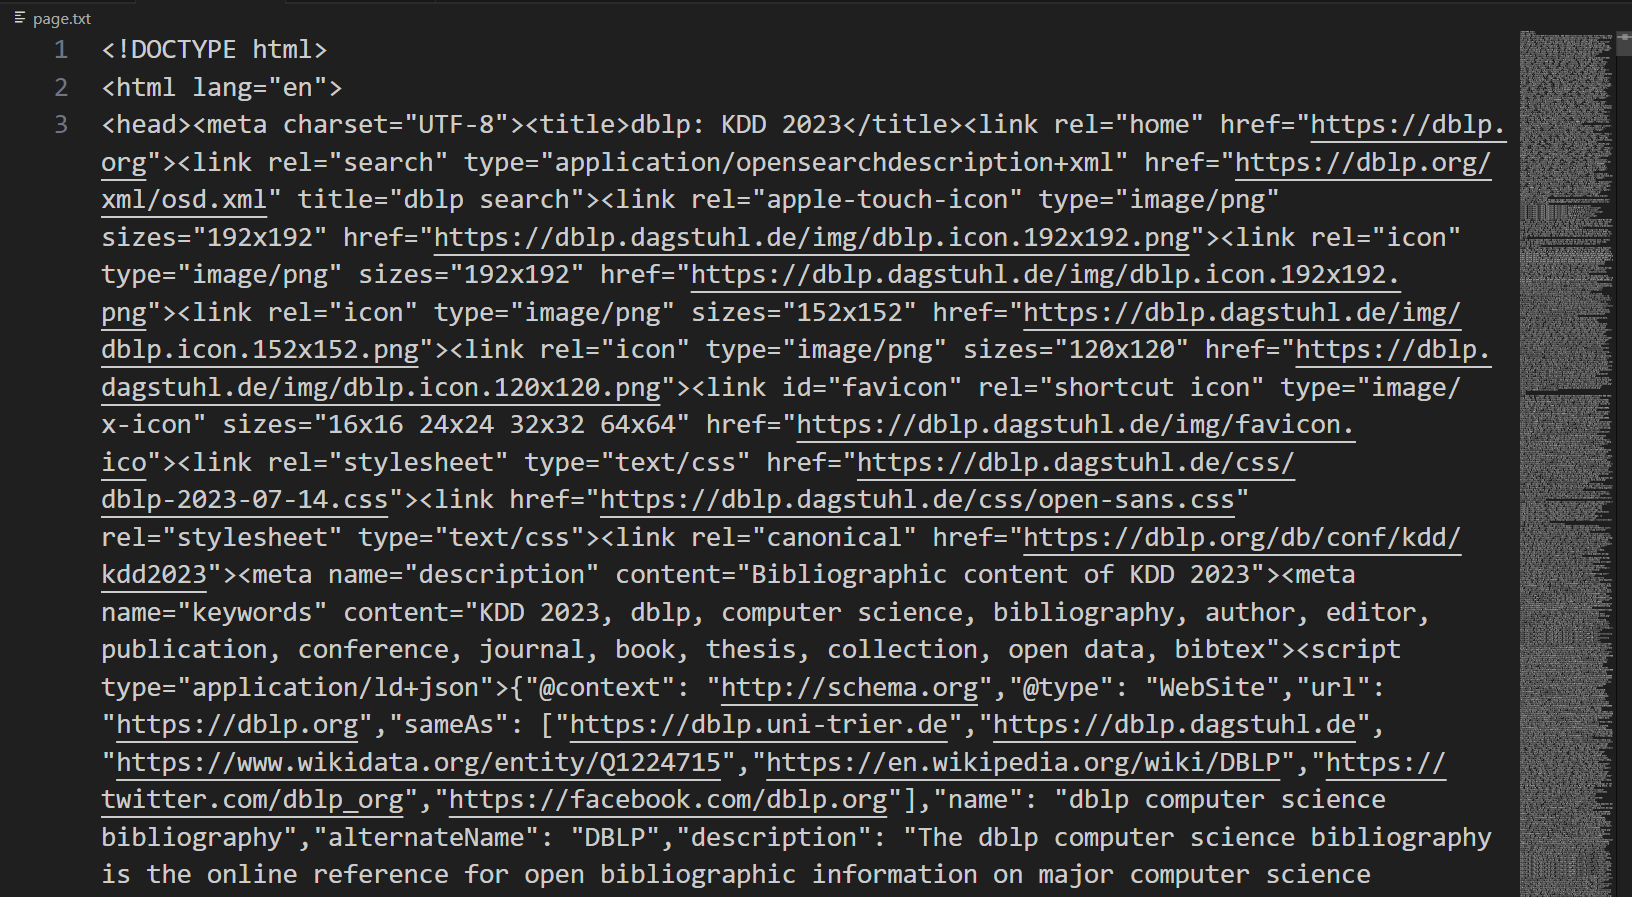
\includegraphics[height=8cm,width=14cm]{1.png}
	\end{figure}
    \section{Task2}
    \subsection{Algorithm Description}
使用\verb|re.findall()|找到所有的\verb|<h2 id="*">| 和\verb|</h2>| 之间的字符串(也即是track的名称)并输出。

\subsection{Results}
\begin{figure}[H]
	\centering 
	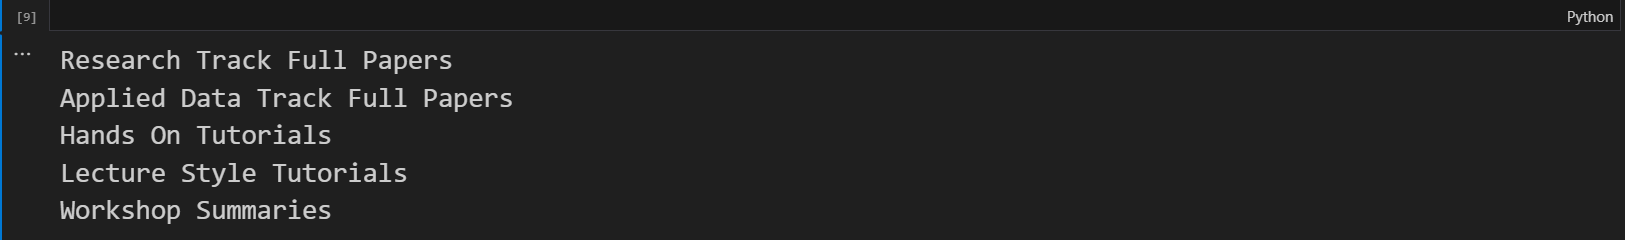
\includegraphics[height=2cm,width=14cm]{2.png}
	\end{figure}
    \section{Task3}
    \subsection{Algorithm Description}
	通过正则表达式从文本文件中提取出 "Research Track Full Papers" 和 "Applied Data Track Full Papers" 两个部分的内容。
	接着划分其中所有相邻\verb|<cite|和\verb|</cite>|之间的内容(即一篇文章的范围)储存到一个字符串元组中,元组的长度即文章的篇数。
	然后定义一个函数\verb|extract_paper_info()| 运用正则表达式提取每篇论文的作者、标题和起始页码、结束页码。
	随后将提取到的论文信息存储在一个包含字典的列表 tracks 中,每个字典包含跟踪名称及其对应的论文列表。
	最后,使用\verb|json.dump()|将tracks列表转换为 JSON 格式,写入\verb|kdd23.json|文件。
	
\subsection{Results}
\begin{figure}[H]
	\centering 
	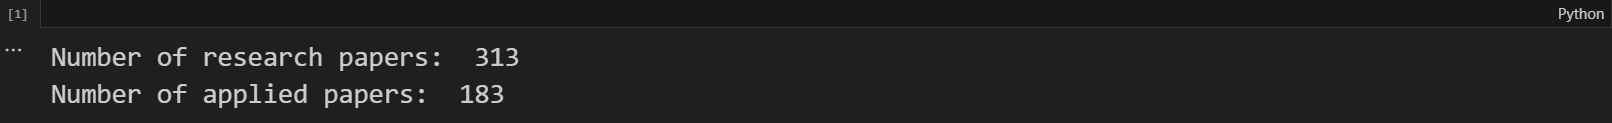
\includegraphics[height=1cm,width=14cm]{3.png}
	\end{figure}
    \section{Task4}

	\subsection{Algorithm Description}
	使用正则表达式识别作者链接、orcID(有多个就爬取所有的)、论文信息。
	提取Research Track Full Papers和Applied Data Track Full Papers两部分的内容,
	并找到前10个\verb|persistent URL:|之间(即一篇文章)的内容。
	遍历每篇文章,使用\verb|requests.get(link)|访问作者链接。
	提取\verb|<li class="underline" title="jump to the 2020s">| 和
	
	\verb|<li class="underline" title="jump to the 2010s">| 之间的内容(即2020年以后发表的文章),
	并根据\verb|</cite>|划分各篇文章的内容,用正则表达式提取年份,
	接着去除所有尖括号之间的内容,把剩下的字符串存为一个字符串元组,
	依次提取作者和题目信息,剩下的所有内容就是出版信息。
	最后将作者、orcID、出版信息和年份以字典形式存储存储到\verb|researchers.json|文件中。

	另外,由于爬虫时频繁请求服务器,曾被网站认定为攻击行为并报错:
	
	\verb|ConnectionResetError: [WinError 10054] 远程主机强迫关闭了一个现有的连接|

	故采取访问后关闭响应和在各个请求之间添加随机延时等待
这两个措施来避免报错。	
\subsection{Results}
\begin{figure}[H]
	\centering 
	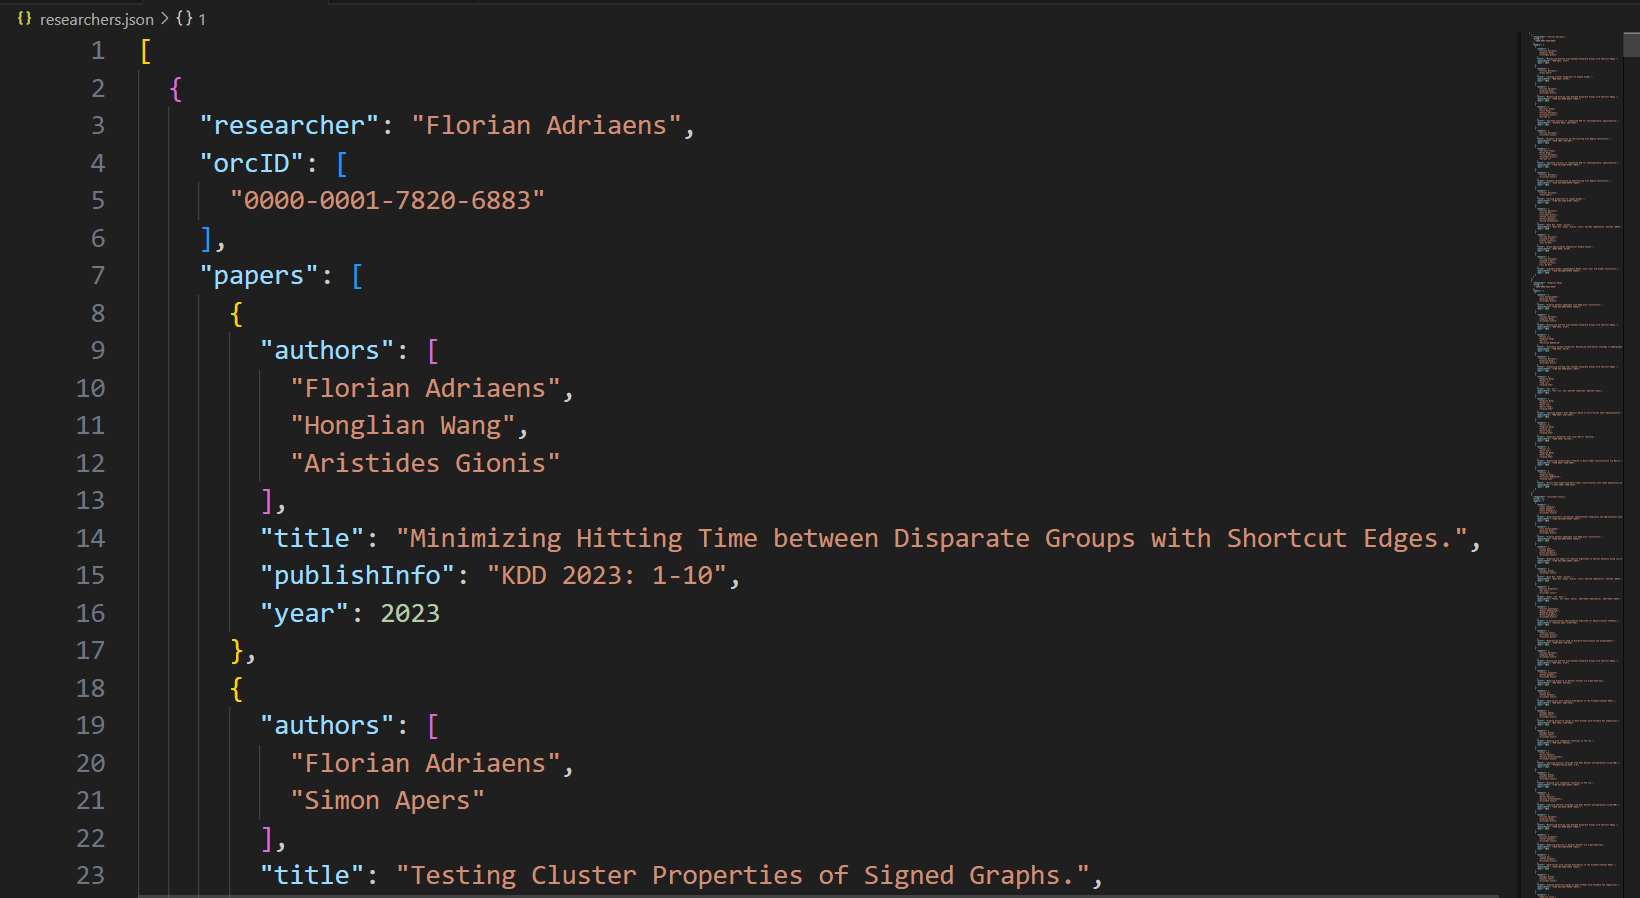
\includegraphics[height=8cm,width=14cm]{4.png}
	\end{figure}

\end{document}